\chapter{Introduction} \label{ch:intro}
The wave of technological advancements named the fourth industrial revolution, has introduced a significant amount of robots into the industrial environment \cite{4_0_Industrial_revolution}. A field expanded upon due to this wave, is human-robot collaboration (HRC). But even with all the collaborative robots made to this date, the level of collaboration used in the industry is still at the coexistence and synchronization levels \cite{HRC_levels}. It is therefore impervious, that more technological advancements are made with the intent of benefiting HRC. Advancements in HRC could pave the way for human-robot interaction both in the industry and outside. The advancements made in the industrial setting could possibly enable the implementation and expansion of robots in other industries, with a new found success. This could be in the medical field, where robots could be used as patient assistants for food delivery or general-purpose task solvers. They could also be used by surgeons as medical assistants during operations.
It could also be within the service industry, where robots could be implemented as robotic waiters that could accomplish tasks given by the customers.
This thesis will focus on reducing complexity in robot control, with the intent of benefiting HRC.
It is therefore hypothesized that a robot controller capable of understanding natural language, is a good proposition for a simplified robot controller. by expanding upon HRC, then this thesis will therefore benefit the technological advancements of the fourth industrial revolution.


\section{Problem formulation}
The objective of this bachelors thesis is to design and develop a system that uses natural language text to control the motion of a 6-DOF manipulator equipped with a parallel gripper. The system must translate natural language input into executable robot commands.
Formulated as a problem formulation, the problem is:

\begin{center}
    \textbf{Problem formulation}
\end{center}
\noindent\fbox{
    \parbox{\textwidth}{
        Can a system be developed to use natural language text commands to control the motion of a 6-DOF robot manipulator equipped with a parallel gripper?
    }
}
\begin{center}
\end{center}


The problem formulation is then divided into sub-tasks, as shown below.
\begin{itemize}
    \item Implementing a language model for Natural Language Processing (NLP).
    \item Designing a parser for translating NLP information into robot executable code.
    \item Designing a constricted set of robot movements that enables the robot to solve tasks.

\end{itemize}

The project is evaluated based on:
\begin{itemize}
    \item In terms of success rate, How well the system interprets natural language instructions.

\end{itemize}

\section{Problem constraint}
The task given in this thesis is solved based on a list of constraints used to set expectations for the project and limit the scope. The first constraint is what kind of natural language input is expected for robot control. This constraint is set to limit the user from using natural language input that would require too much processing complexity to be solved. Like the input \textit{'cook an omelete'}. Another constraint is based on the hardware limit for this project. The constraints given due to the reasons mentioned are shown as follows:

\begin{itemize}
    \item The Natural Language Processing is limited to support non-contextual natural language formulations.
    \item Only a finite list of actions is supported by the robot. and not all natural language input can be processed, disregarding contextuality.
    \item The hardware is limited to a UR5e robot arm\footnote{https://www.universal-robots.com/da/produkter/ur5-robot} and a Robotiq Hand-E gripper\footnote{https://robotiq.com/products/hand-e-adaptive-robot-gripper}.
\end{itemize}

With these constraints, the scope of the thesis has been placed alongside the overall problem. The next section will outline the contents of each chapter in the thesis.

\section{Thesis outline}
The thesis will focus on solving the task given in the problem formulation. Figure \ref{fig:thesis_outline} shows a system overview.

\begin{figure}[ht]
    \centering
    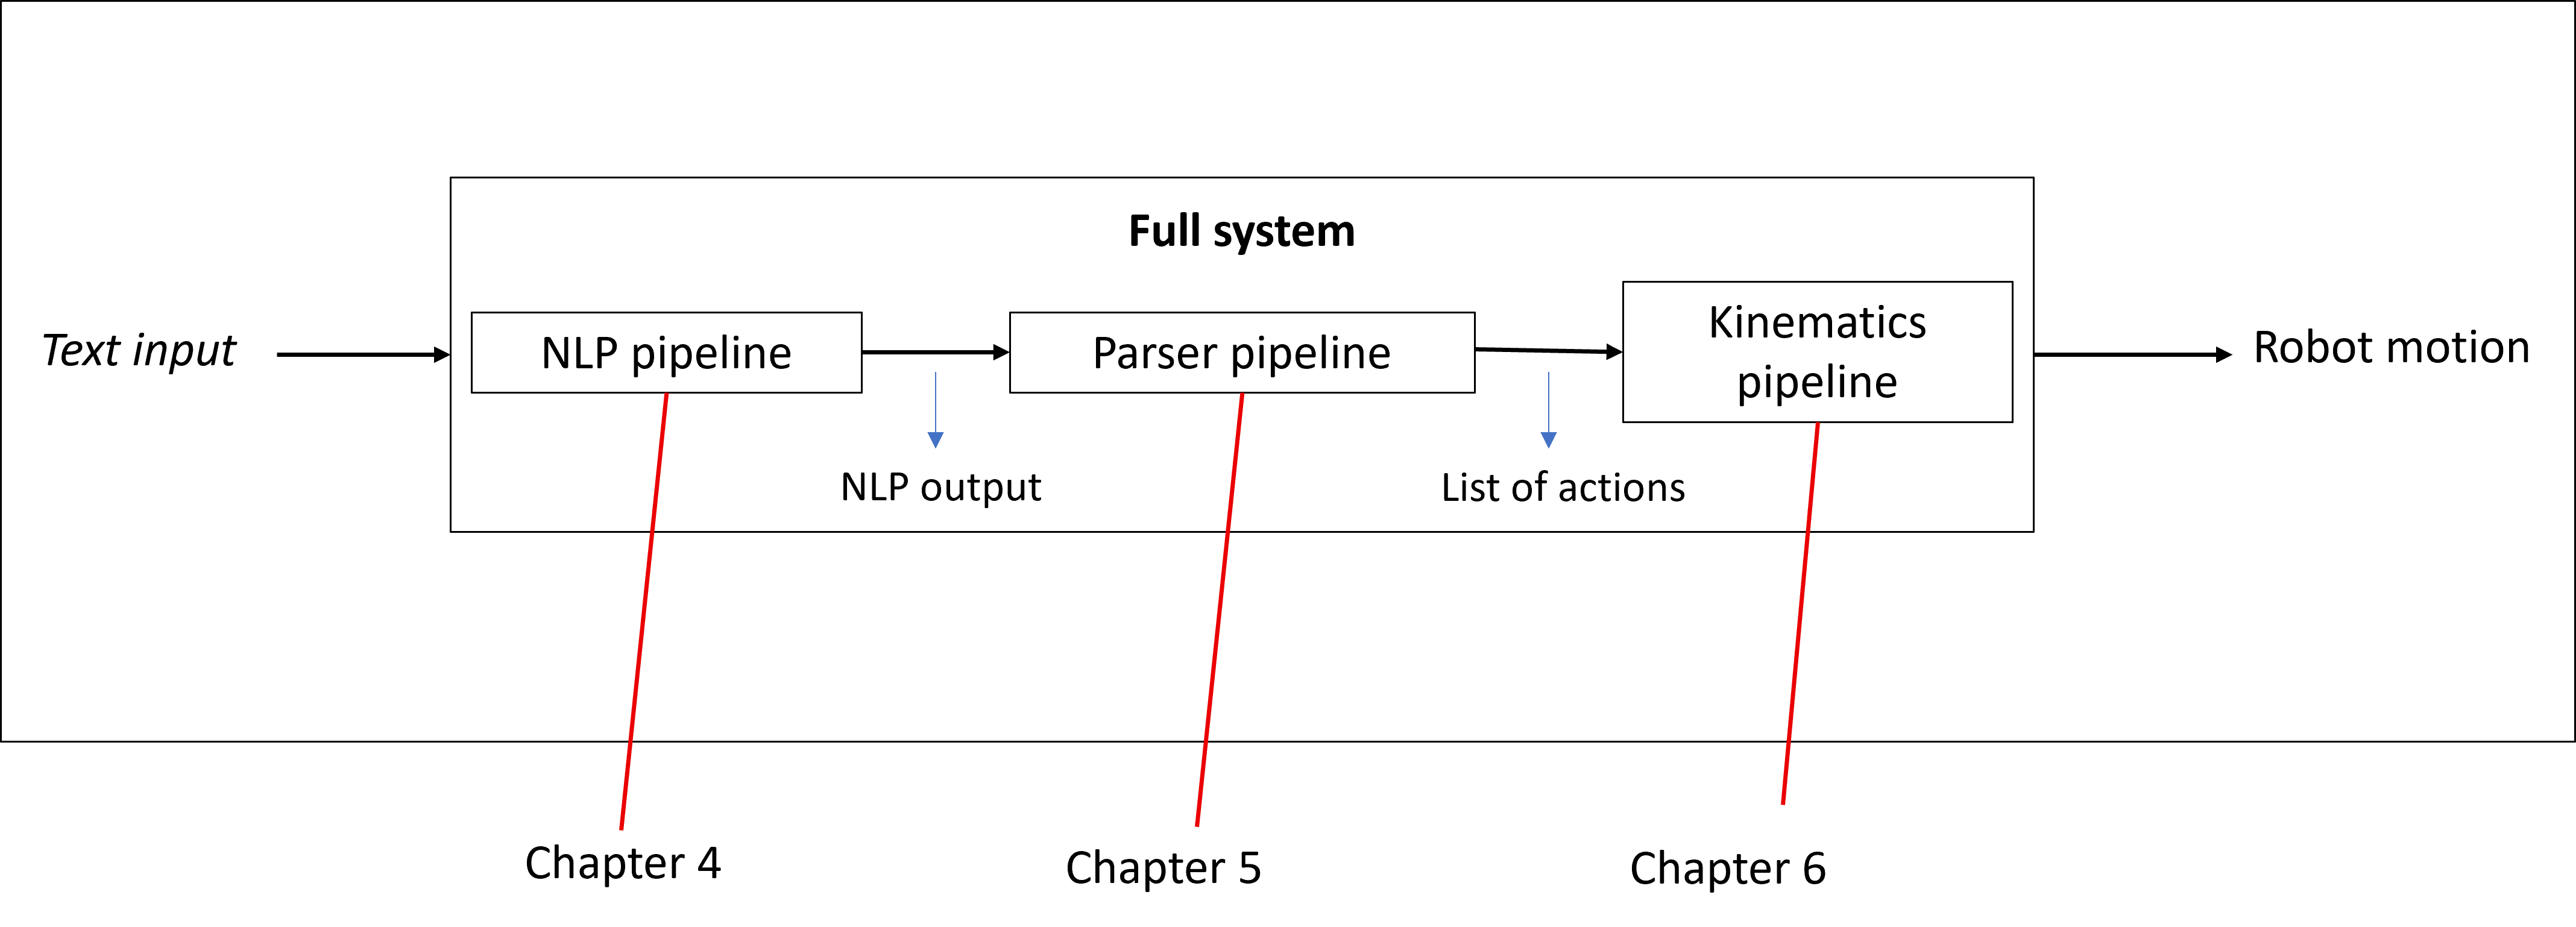
\includegraphics[width=15cm]{img/thesis_outline.png}
    \caption{Figure shows an illustration of the whole system, along with chapter referenes.}
    \label{fig:thesis_outline}
\end{figure}

The content of the thesis is outlined in the list below.
\begin{itemize}
    \item Chapter \ref{ch:background} is the background for robot control using NLP. This information serves as inspiration for how the problem formulation is solved.
    \item Chapter \ref{ch:overview} gives an overview of the system design structure. It is used to describe the input-output structure, the motion planning structure and the user interface of the system.
    \item Chapter \ref{ch:NLP} as shown in figure \ref{fig:thesis_outline} is the first chapter describing a sub-pipeline. This chapter analyzes natural language command text, and describes which NLP tools is used in this thesis. Afterwards the chapter describes the output from this pipeline.
    \item Chapter \ref{ch:parser_pipeline} explains the parser pipeline, and how it processes the output from the NLP pipeline into actions executable by the robot manipulator.
    \item Chapter \ref{ch:Kinematics_intro} introduces the kinematics of the UR5e robot arm and the Robotiq Hand-E gripper. This chapter explains how the robot is modelled and how it is controlled.
    \item Chapter \ref{ch:eval} is an evaluation of the effectiveness of the system based on the evaluation criteria given in the problem formulation. 
    \item The last three chapters are the discussion, conclusion and future work of the thesis.
\end{itemize}

The next chapter introduces the background for the thesis.